
%% This file represents a sample second chapter of the main body of the dissertation
%%
%%**********************************************************************
%% Legal Notice:
%% This code is offered as-is without any warranty either
%% expressed or implied; without even the implied warranty of
%% MERCHANTABILITY or FITNESS FOR A PARTICULAR PURPOSE!
%% User assumes all risk.
%% In no event shall any contributor to this code be liable for any damages
%% or losses, including, but not limited to, incidental, consequential, or
%% any other damages, resulting from the use or misuse of any information
%% contained here.
%%**********************************************************************
%%
%% $Id: chapterTwo.tex,v 1.4 2006/08/24 21:12:59 Owner Exp $
%%


% A first, optional argument in [ ] is the title as displayed in the table of contents
% The second argument is the title as displayed here.  Use \\ as appropriate in
%   this title to get desired line breaks
\chapter[Background]{Background}

\section{Intel Optane DC Persistent Memory}

Intel Optane Persistent Memory (PMM) represents a significant advancement in persistent memory technology, bridging the gap between dynamic random-access memory (DRAM) and storage devices \cite{scargall2020pmem}. As a result, it has been applied to speed up data-intensive workloads in both commercial and research settings, such as in-memory databases, virtualization software, and high-performance computing \cite{peng2020demystifying,SolveMod32:online}. This section provides an overview of the architecture, features, benefits, and applications of Intel Optane PMM.

\subsection{Overview of Intel Optane DC PMM}

\begin{figure}[ht]
    \centering
    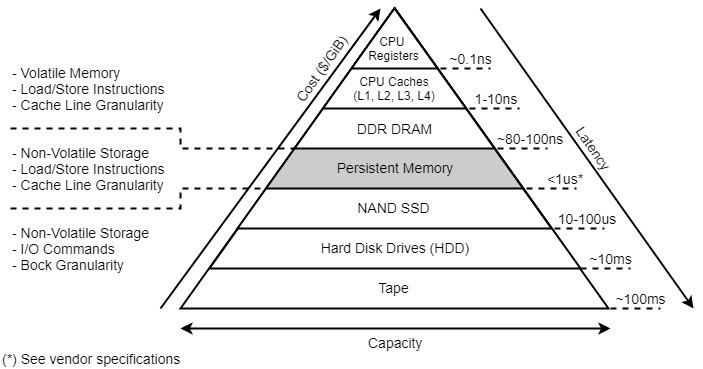
\includegraphics[scale=0.6]{images/pmem_storage_pyramid.jpg}
    \caption{Memory Hierarchy. Taken from \cite{Introduc86:online}}
    \label{fig:pmem_storage_pyramid}
\end{figure}

Persistent memory, also referred to as Non-Volatile Memory (NVM), represents a significant evolution in the memory/storage hierarchy (Figure \ref{fig:pmem_storage_pyramid}), addressing the performance and capacity gap between dynamic random-access memory (DRAM) and traditional storage mediums. This innovative technology combines the characteristics of both DRAM and storage, offering the speed of DRAM and the non-volatile nature of storage devices \cite{scargall2020pmem}.

Like DRAM, persistent memory is available in the form of Dual In-line Memory Modules (DIMMs), which are directly connected to the memory bus. This direct connection enables applications to access persistent memory with the same ease as traditional DRAM, eliminating the need for frequent data transfers between memory and storage. However, unlike DRAM, persistent memory DIMMs provide significantly greater capacity and retain data even when power is removed, thereby enhancing system performance and enabling fundamental changes in computing architecture \cite{rudoff2017persistent,scargall2020pmem}.

Intel Optane DC Persistent Memory Module (Optane PMM) stands at the forefront of commercial implementations of persistent memory technology, leveraging Intel's innovative 3D-XPoint technology. Upon its introduction, the Optane PMM offers substantial capacities up to 512GiB and is exclusively supported by Intel Cascade Lake platform. Each processor within this platform is equipped with two integrated memory controllers (iMCs), with each iMC supporting three channels. This architecture seamlessly integrates Optane PMM with DRAM, allowing users to deploy up to one Optane PMM per channel and up to six per CPU socket, thereby enabling extensive memory capacities of potentially up to 3TiB per socket \cite{yang2020empirical,izraelevitz2019basic}.

Similar to conventional DRAM DIMMs, Optane PMMs are positioned on the memory bus and connect directly to the processor's iMC. The communication protocol between the iMC and the Optane PMM is depicted in Figure \ref{fig:optane_communication}.  Communication between the iMC and the Optane PMM occurs via the DDR-T protocol, adapted for persistent memory and operating at cache line granularity (64B). Initial memory access to the Optane PMM is coordinated by the onboard Controller, which manages access to the 3D-XPoint media. Analogous to SSDs, the Optane PMM conducts address translation for wear-leveling and bad block management, facilitated by the maintenance of an address indirection table (AIT). Following translation, access to the storage media occurs. Notably, with 3D-XPoint access granularity set at 256B, the controller converts 64-byte accesses into 256-byte accesses, inducing write amplification. To mitigate this, the Controller incorporates a 16KB write-combining buffer to merge adjacent writes \cite{yang2020empirical,izraelevitz2019basic,wu2020ribbon}.

\begin{figure}[ht]
    \centering
    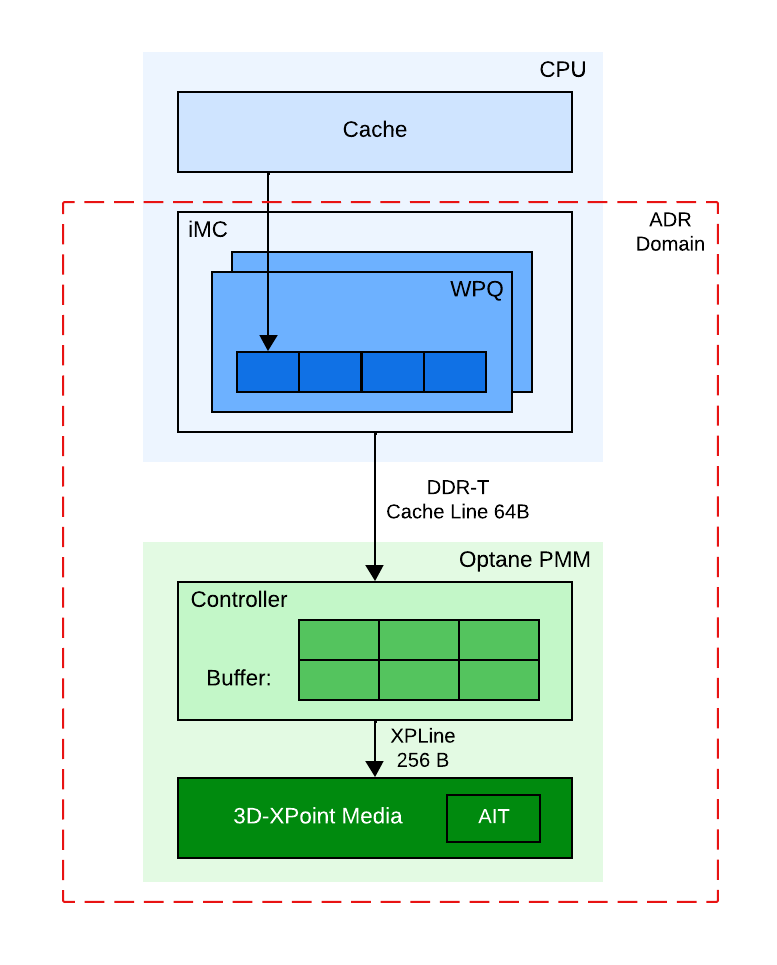
\includegraphics[scale=0.7]{images/optane-communication.png}
    \caption{Communication between iMC and Optane PMM}
    \label{fig:optane_communication}
\end{figure}

To ensure data persistence, Intel platforms integrate the iMC and Optane PMM within the asynchronous DRAM refresh (ADR) domain. Intel's ADR feature ensures that CPU stores that reach the ADR domain will survive a power failures \cite{yang2020empirical}. The iMC manages read and write pending queues for each Optane PMM, with the ADR domain encompassing the write pending queue. Once data reaches the write pending queue, ADR ensures its persistence within Optane PMM in the event of power failures. The ADR domain excludes the CPU caches, necessitating additional steps beyond simply executing a store instruction to ensure data persistence. To achieve this, CPU stores must be continually flushed using specialized instructions provided by Intel's Instruction Set Architecture (ISA), including \textrm{CLFLUSH}, \textrm{CLFLUSHOPT}, and \textrm{CLWB} \cite{yang2020empirical,izraelevitz2019basic,rudoff2017persistent}.

\subsection{Performance Characterization}
Previous studies \cite{yang2020empirical,izraelevitz2019basic} conducted an empirical performance assessment of Optane PMM, revealing its nuanced behavior compared to DRAM. They observed that Optane's performance varies significantly depending on specific access patterns, including access size, type, and concurrency level. Notably, they found that Optane's read latency is three times slower than that of DRAM, primarily due to Optane's longer media latency. However, sequential access patterns demonstrate notably improved latency, indicating Optane PMM's capability to consolidate adjacent requests into single 256-byte accesses. The study also highlights that Optane PMM achieves a maximum random read bandwidth of 6.6 GB/s and a write bandwidth of 2.3 GB/s. Moreover, sequential access further enhances bandwidth performance, exhibiting up to a fourfold increase \cite{yang2020empirical,izraelevitz2019basic}.

An insightful observation highlighted by Izraelevitz et al. \cite{izraelevitz2019basic} is that Optane PMM's bandwidth can become saturated when utilized in real-world multi-threaded applications, thereby introducing performance overhead. This phenomenon arises due to Optane PMM's inability to scale performance proportionally with increased thread count, primarily due to contention occurring within the processor's integrated memory controller (iMC) and Optane PMM's buffer. Contentious conditions within the buffer exacerbate the frequency of evictions and write-backs to the 3D-XPoint media, resulting in Optane writing more data internally than what the application necessitates. Furthermore, given Optane PMM's slightly slower performance compared to DRAM, the slower drainage of write pending queues by Optane PMMs introduces head-of-line blocking effects. As the number of threads concurrently accessing Optane PMM increases, contention on the device escalates, heightening the likelihood of the processor experiencing blocking while awaiting completion of previous store operations \cite{yang2020empirical}.

\subsection{Operating Modes and Applications}

Intel Optane persistent memory (PMem) offers two distinct operating modes: Memory mode and App Direct mode.

In Memory mode, Optane PMem serves as a high-capacity main memory without persistence. In this configuration, DRAM is concealed from users and acts solely as a cache for Optane PMem, seamlessly managed by the operating system \cite{yang2020empirical}. 

Conversely, in App Direct mode, Optane PMMs are directly exposed to the operating system as independent persistent memory devices, thus enabling their utilization for persistent storage \cite{izraelevitz2019basic}. Functionally, the operating system perceives DRAM and Optane PMem as distinct memory pools, with the latter offering data persistence. Applications can access Intel Optane persistent memory through direct load/store operations or via a file system configured with the \textrm{dax} (direct access) option. Such a file system is termed as a PM-aware file system, facilitating direct access to persistent memory without relying on the page cache \cite{rudoff2017persistent,Speeding28:online}.

In the context of this thesis, Optane PMem is exclusively employed in App Direct Mode, coupled with a PM-aware file system to harness its storage capabilities.

\subsection{Programming}

In the realm of persistent memory technology, maintaining data consistency across runtime and system reboots is essential. To address this challenge, prior research underscores the necessity for applications leveraging persistent memory to implement transactions that are atomic, consistent, thread-safe, and resilient to system failures—a paradigm akin to ACID transactions in database systems. However, achieving such robustness in real-world scenarios poses significant complexity. Recognizing this, Intel has developed the Persistent Memory Development Kit (PMDK) to tackle this challenge \cite{scargall2020pmem,rudoff2017persistent}.

PMDK comprises a comprehensive suite of libraries and tools tailored for both application developers and system administrators, aiming to streamline the management and utilization of persistent memory devices. Drawing on the SNIA NVM Programming model \cite{NVMProgr73:online} as its foundation, these libraries extend its capabilities to varying extents. Some libraries offer simplified wrappers around operating system primitives, facilitating ease of use, while others provide sophisticated data structures optimized for persistent memory usage \cite{scargall2020pmem}.

In the scope of this thesis, we leverage pmemkv \cite{GitHubpm66:online}, a persistent local key-value store provided by PMDK. Designed with cloud environments in mind, pmemkv complements PMDK's suite of libraries with cloud-native support, abstracting the intricacies of programming with persistent memory through a familiar key-value API. Notably, pmemkv distinguishes itself from traditional key-value databases by enabling direct access to data. This means that reading data from persistent memory circumvents the need for copying it into DRAM—an approach that significantly enhances the performance of applications leveraging persistent memory \cite{scargall2020pmem}.

\section{Serverless Computing}
Serverless computing, a prominent execution model within cloud computing, revolutionizes the deployment process by allowing developers to deploy code without the need for provisioning or managing server infrastructure. Although termed "serverless," this model still utilizes servers provided by cloud vendors to execute developers' code. However, the distinguishing feature lies in the abstraction of infrastructure management from the developer's perspective. Developers no longer concern themselves with resource provisioning, scaling, fault tolerance, monitoring, or security patches; instead, they focus solely on code development. Cloud providers take on the responsibility of handling these infrastructure-related tasks on behalf of their customers. Consequently, developers are charged based on the execution time and resources consumed during their code invocations, offering a pay-per-use billing model \cite{jonas2019cloud,romero2021faat,klimovic2018pocket}.

Serverless computing has witnessed remarkable growth in recent years, emerging as a prominent paradigm for cloud application development. While it was originally developed for web microservices and IoT, its elasticity and billing granularity make it appealing for other types of applications. Recent studies have highlighted the benefits of transitioning more applications to serverless computing platforms, with applications focused on video processing \cite{fouladi2017encoding}, data analytics \cite{gimenez2019framework,carver2020wukong,klimovic2018pocket}, machine learning \cite{carreira2019cirrus,feng2018exploring}, and storage applications \cite{10.14778/3587136.3587139,jonas2019cloud}.

\subsection{Funtion-as-a-Service (FaaS)}
At the heart of serverless computing lies Function-as-a-Service (FaaS), introduced by AWS Lambda in 2015. Since then, various commercial and open-source alternatives have emerged, including Google Cloud Functions, Azure Functions, Apache OpenWhisk, and others. FaaS enables developers to express application logic as stateless functions written in high-level languages such as Java, Python, C, or C++. These functions, known as serverless functions, are packaged together with their dependencies and submitted to the serverless platform. Additionally, developers associate events with each serverless function, such as HTTP requests, file uploads, database triggers, and more. Upon the occurrence of a trigger, the cloud provider promptly executes the associated serverless function, offering a scalable and event-driven approach to application development and deployment \cite{AWSLambd40:online,AzureFun49:online,CloudFun3:online,ApacheOp28:online}.

\subsubsection*{Workload Characterization}
Previous research has underscored the dynamic and unpredictable nature of Function-as-a-Service (FaaS) workloads within serverless computing environments. Typically, applications in serverless computing are composed of interconnected serverless functions, each serving a specific logical purpose. Analyzing these workloads often involves examining real-world FaaS provider logs to discern patterns and characteristics. Cloud providers face significant challenges in predicting the next function invocation due to the diverse array of triggers employed by applications. Moreover, the heterogeneity of these applications results in substantial variations in invocation frequency, data access sizes, and usage patterns. Data access sizes can range from mere bytes to gigabytes, while invocation frequencies can span several orders of magnitude, with some functions being infrequently called. Learning the invocation patterns of rarely invoked functions is particularly challenging. Additionally, a significant portion of data accesses exhibit bursty behavior, leading to rapid surges in I/O requests as multiple function instances are dynamically spun up to meet application demands. This phenomenon often results in short-lived bursts of intense activity within applications \cite{shahrad2020serverless,romero2021faat,klimovic2018pocket}.

\subsection{Storage for FaaS}

Serverless providers enforce a restriction on direct communication between serverless functions, necessitating the adoption of remote storage mechanisms for data interchange among them \cite{jonas2019cloud,klimovic2018pocket,romero2021faat}.

One approach to facilitate data exchange between serverless functions is through the utilization of serverless storage, a framework within cloud computing that abstracts the intricacies of managing storage infrastructure from developers. With serverless storage, developers harness storage services provided by cloud vendors like AWS S3, Google Cloud Storage, Azure Blob Storage, AWS DynamoDB, and others. These services empower developers to store and retrieve data via APIs or SDKs without the burden of managing servers or storage clusters. Moreover, serverless storage services offer features such as automatic scaling, data durability, and pay-per-use pricing models, enabling developers to seamlessly adjust their storage resources in line with demand without the need for upfront provisioning or capacity planning. This scalability is of paramount importance for applications characterized by fluctuating storage requirements or unpredictable workloads  \cite{CloudObj90:online,AmazonDy45:online,DeCandia2007,AzureBlo83:online,CloudSto52:online,Datastor50:online,AzureCos63:online}.

Despite the high scalability of existing serverless storage solutions, they are primarily optimized for durability rather than performance \cite{jonas2019cloud,klimovic2018pocket,10.14778/3587136.3587139}. Studies have demonstrated that object-based storage solutions like AWS S3 may exhibit latencies of up to 10 milliseconds for small object reads or writes \cite{PublicCl96:online}. Similarly, key-value databases such as AWS DynamoDB, Google Cloud Datastore, and Azure Cosmos provide high throughput but may entail high expenses and lengthy scaling processes \cite{jonas2019cloud}.

In scenarios demanding enhanced performance, developers may opt for in-memory key-value stores like AWS ElastiCache \cite{AmazonEl88:online}. These solutions offer low access latencies and high throughput but incur higher costs associated with DRAM. Additionally, they do not provide persistence, meaning that data is not retained in the event of a system failure. However, a notable drawback is their lack of autoscaling capabilities, necessitating manual management and scaling of clusters when integrated with serverless functions \cite{jonas2019cloud,klimovic2018pocket,10.14778/3587136.3587139}.

\subsection{Service Level Agreements}
%citations \cite{DeCandia2007,180275}
Service level agreements (SLAs) are integral to cloud storage as they establish the terms and conditions governing the quality of service between cloud providers and customers. These agreements, formalized through SLAs, represent negotiated contracts wherein both parties delineate system-related attributes, including the client's anticipated request characteristics and the expected performance of the storage service under these conditions. SLAs serve to define the repercussions for any deviation from the predetermined service levels, often entailing service credits, refunds, or other forms of redress. Such measures incentivize providers to fulfill their obligations and redress any disruptions or deficiencies in service promptly \cite{DeCandia2007,180275,tariq2020sequoia}.

In the realm of storage services, latency and throughput-related SLAs are of paramount importance. While conventional practice often involves describing performance SLAs using mean or median metrics, these measures may not adequately ensure a consistently positive user experience across all customers. Instead, a more effective approach involves assessing performance SLAs in terms of tail (99th) percentiles, thereby prioritizing the resolution of exceptional cases and optimizing service quality for all users \cite{DeCandia2007}.

\section{Reinforcement Learning}

Reinforcement Learning (RL) is a subfield of machine learning concerned with learning optimal decision-making policies through interactions with an environment \cite{sutton2018reinforcement}. 

\subsection{Overview of Reinforcement Learning}
The fundamental concept underlying RL is the notion of an agent, which takes actions in an environment and receives feedback in the form of rewards, indicating the quality of its decisions. The agent's objective is to learn a policy that maximizes cumulative rewards over time. Moreover, the agent is not provided with explicit instructions on which actions to take; instead, it must discover the actions that lead to the highest rewards by trying them.

\begin{figure}[ht]
    \centering
    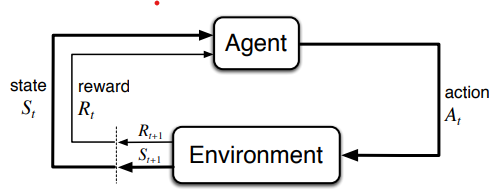
\includegraphics[scale=1]{images/rl-workflow.png}
    \caption{RL Workflow}
    \label{fig:sutton_rl_workflow}
\end{figure}

Figure \ref{fig:sutton_rl_workflow} presents a schematic representation of a standard reinforcement learning scenario. In discrete time steps, the agent perceives the current state $s_t$ from the set of all possible states $S$. It then selects an action $a_t$ from the available actions $A(s_t)$ in the current state. The environment transitions to a new state $s_{t+1}$, and the agent receives a reward $r_t$ associated with the transition $(s_t, a_t, s_{t+1})$.

The agent's behavior is governed by its policy, which maps perceived states to actions. The ultimate aim is to learn an optimal or near-optimal policy that maximizes the cumulative reward. 


\subsection{Q-Learning}

One of the foundational algorithms in RL is Q-Learning, introduced by Watkins in 1989 \cite{watkins1989learning}. The algorithm belongs to the class of model-free RL algorithms, meaning it learns directly from experience without requiring a model of the environment dynamics \cite{russel2020ai}.

At the core of Q-Learning is the Q-value function, denoted as $Q(s, a)$, which represents the expected cumulative reward the agent will receive by taking action $a$ in state $s$ and following an optimal policy thereafter. The objective of Q-Learning is to iteratively update the Q-values based on observed transitions and rewards, eventually converging to the optimal Q-values that maximize long-term rewards.

The Q-Learning algorithm proceeds as follows: the agent interacts with the environment by selecting actions based on its current estimate of the Q-values. Upon taking an action, the agent observes the resulting reward and the next state. It then updates the Q-value of the previous state-action pair using the observed reward and the estimated value of the next state.

The Q-value update rule in Q-Learning is based on the Bellman equation, which expresses the relationship between the Q-values of successive states \cite{russel2020ai}:

\[
Q(s, a) \leftarrow (1 - \alpha) \cdot Q(s, a) + \alpha \cdot \left( r + \gamma \cdot \max_{a'} Q(s', a') \right)
\]

Here, $\alpha$ is the learning rate, determining the extent to which new information overrides the old one, and $\gamma$ is the discount factor, representing the importance of future rewards relative to immediate rewards. The term $r + \gamma \cdot \max_{a'} Q(s', a')$ is known as the temporal-difference (TD) target, combining the immediate reward $r$ with the discounted maximum Q-value of the next state $s'$ \cite{russel2020ai}.

% Q-Learning, a model-free reinforcement learning algorithm, is employed by the agent to determine the best action given the current state. The agent evaluates action quality using a quality-function (Q-function) $Q(s, a)$, representing the expected total discounted reward if the agent selects action $a$ in state $s$ and acts optimally thereafter. 

% One of the foundational algorithms in RL is Q-Learning, introduced by Watkins in 1989 \cite{watkins1989learning}. Q-Learning is a model-free algorithm that learns the value of taking an action in a particular state, known as the Q-value, and iteratively refines these values through experience. The Q-value represents the expected cumulative reward the agent will receive by taking an action in a given state and following an optimal policy thereafter.

% The Q-Learning algorithm (illustrated in Figure \ref{algo:q_learning}) involves iterative updates to the Q-function. At each step, the agent selects an action, observes the reward and new state, and then applies one-step Q-learning. The update is governed by the Q-learning formula, where the learning rate ($\alpha$) determines the extent to which new information overrides old data. This learned Q-function approximates the optimal Q-function, irrespective of the policy being followed.

\subsection{Function Approximation using Linear Regression Models}

One of the key advantages of Q-Learning is its simplicity and ease of implementation. It requires only a table to store the Q-values, making it computationally efficient for small state and action spaces. However, Q-Learning faces challenges in environments with large state spaces, as maintaining a lookup table becomes infeasible due to memory and computational constraints.

Function approximation is a fundamental technique in reinforcement learning (RL) aimed at approximating the Q-Value function when dealing with large state or action spaces where tabular representations become impractical \cite{russel2020ai}. This approach allows RL agents to generalize from observed states to unseen states, facilitating decision-making in unexplored regions of the state space.

In the context of RL, linear regression models are commonly used for function approximation \cite{sutton2018reinforcement}.  These models approximate the Q-value function by leveraging a weighted linear combination of features, with each feature capturing a distinct aspect of the state space. Employing gradient-descent methods, notably stochastic gradient descent, enables iterative refinement of the parameters governing the linear function, aimed at minimizing a predefined loss function. This iterative optimization process empowers the model to progressively enhance its predictive accuracy and capture intricate patterns within the state-action space.

Hyperparameter tuning is a critical aspect of training linear regression models in RL \cite{bergstra2012random}. Hyperparameters, such as the learning rate, regularization strength, and feature scaling, significantly impact the performance and convergence of the models. A systematic approach to hyperparameter tuning involves experimenting with different combinations of hyperparameters, evaluating the performance of the trained models on a validation set, and selecting the optimal hyperparameters based on predefined criteria, such as validation error or performance metrics \cite{russel2020ai}.

\subsection{Exploration-Exploitation Tradeoff}

The exploration-exploitation tradeoff poses a significant challenge in reinforcement learning \cite{sutton2018reinforcement}. The agent must strike a balance between exploring unfamiliar actions to gather information and exploiting known actions for immediate rewards. Finding this balance is crucial for effective learning and task performance, as the agent gradually favors actions with higher expected rewards.

One classic strategy for balancing exploration and exploitation is the epsilon-greedy (e-greedy) algorithm \cite{sutton2018reinforcement}. The e-greedy policy selects the action that maximizes the estimated value with probability $1 - \epsilon$ (exploitation) and selects a random action with probability $\epsilon$ (exploration). This approach ensures that the agent continues to explore the environment while gradually exploiting more rewarding actions as it gains knowledge.

Decayed e-greedy methods aim to strike a balance between exploration and exploitation by gradually reducing the exploration rate $\epsilon$ as the agent gains more experience or as the training progresses \cite{sutton2018reinforcement}. This decay encourages the agent to explore the environment more extensively in the early stages of learning while gradually shifting towards exploitation as it becomes more knowledgeable.

\subsection{Reward shaping}

Reward shaping is a technique in reinforcement learning (RL) aimed at accelerating learning by modifying the reward signal provided to the agent. Traditional RL algorithms rely solely on sparse reward signals, which can make learning slow and inefficient, especially in complex environments. Reward shaping addresses this issue by providing additional, shaped rewards that guide the agent towards desirable behaviors. These shaped rewards are designed to provide more informative feedback to the agent, encouraging it to explore the state-action space more effectively. However, reward shaping must be carefully designed to avoid unintended consequences such as overfitting to the shaped rewards or incentivizing undesirable behaviors \cite{russel2020ai}.
